\section*{CHAPTER 4: SIMULATION AND RESULTS}
\addcontentsline{toc}{section}{\numberline{}CHAPTER 4: SIMULATION AND RESULTS}
\setcounter{section}{4}
\setcounter{subsection}{0}
\setcounter{figure}{0}
\setcounter{table}{0}

In this project, we're utilized the power of Python and the convenient jupyter notebook to simulate the 64 QAM OFDM system. Full notebook can be seen at the Appendix.

\subsection{Configurations and Parameters set up}

\begin{enumerate}
    \item $K = 64$ : The number of subcarriers, describes how many subcarriers are available in the OFDM system.
    \item $CP = K//$4 : The length of the cyclic prefix, denotes the number of samples that are copied from the end of the modulated block to the beginning, to yield a cyclic extension of the block.
    \item $P = 8$ : The number of pilots in the OFDM symbol, describes how many carriers are used to transmit known information (i.e. pilots). Pilots will be used at the receiver to estimate the wireless channel between transmitter and receiver.
    \item $pilotValue = 3+3j$ : The known value each pilot transmits.
    \item $\mu = 6$ :Since we simulating 64QAM transmission, we need to define $\mu = \log_{2} 64$ bits per symbol
    \item $SNRDB = 20$ : Signal-to-Noise Ratio in dB, that should occur at the receiver.
\end{enumerate}

After that, we need to define some index sets that describe which carriers transmit pilots and which carriers contain payload.

\begin{figure}[htbp]
    \centering
    
\includegraphics[width=\linewidth]{../Source/results/carrier_index}
    \caption{The Carriers transmit pilots and which carriers contain payload}
    \label{carrier_index}
\end{figure}

Furthermore, the mapping from groups of 6 bits to a 64QAM constellation symbol shall be defined in mapping table.

\begin{figure}[htbp]
    \centering
    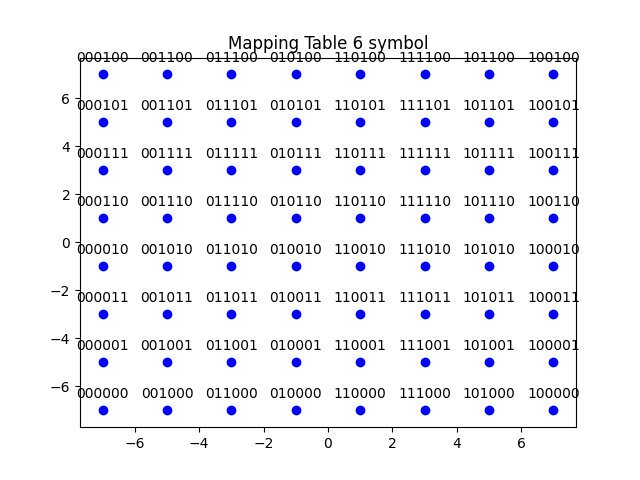
\includegraphics[width=\textwidth]{../Source/results/mapping}
    \caption{64-QAM Constellation with gray-mapping}
    \label{mapping}
\end{figure}

In Figure \ref{mapping}, we have plotted the 64-QAM constellation, along with the bit-labels. In Gray-mapping, two adjacent constellation symbols differ only by one bit and the other 5 bits remain the same. This technique helps to minimize bit-errors, in case a wrong constellation symbol is detected: Most probably, symbol errors are "off-by-one" errors, i.e. a symbol next to the correct symbol is detected. Then, only a single bit-error occurs.

Let us now define the wireless channel between transmitter and receiver. Here, we use a simple two-tap multipath channel with given impulse response channelResponse. Also, we plot the corresponding frequency response. As seen in Figure \ref{channel}, the channel is frequency-selective.

\begin{figure}[htbp]
    \centering
    \includegraphics[width=\textwidth]{../Source/results/channel}
    \caption{64-QAM Constellation with gray-mapping}
    \label{channel}
\end{figure}

\subsection{OFDM Transmitter}

Now, that we have defined the necessary parameters for our OFDM example, we need some data for testing. Here we using a 3 channel 256x256 bitmap image (Figure \ref{input}).

\begin{figure}[htbp]
    \centering
    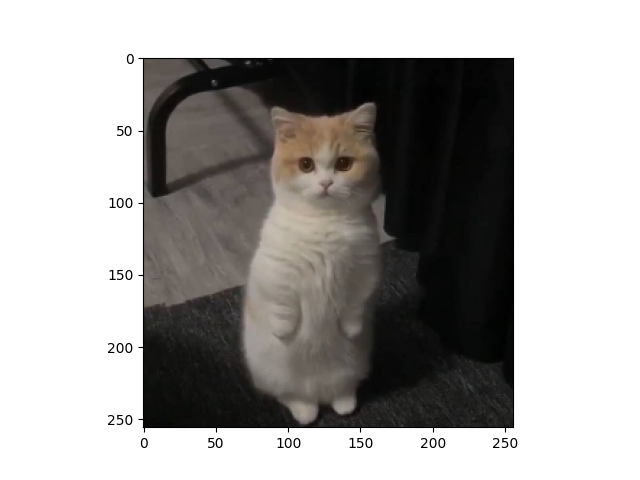
\includegraphics[width=\textwidth]{../Source/results/input}
    \caption{The input source of the OFDM Transmitter}
    \label{input}
\end{figure}

We first need to get all the pixels value (from all 3 channels) and lay them in a 1D array. this array is gonna have a size of $width*height*channel = 256*256*3 = 196608$ (bytes). The pixels value is in decimal, we need to convert it into binary.

Subsequently, we add the CRC (Cyclic redundancy check) \cite{crc} to the end of each byte. The CRC is serve as a way to check for errors. Basically, the  generator at the transmitter consists of 4 steps:

\begin{enumerate}
    \item Find the length of the devisor (key) $L$
    \item Append $L-1$ bits to the original byte
    \item Perform binary division operation to get $quotient$ and $remainder$
    \item Remainder of the division = $CRC$
\end{enumerate}

Since we choose the key value of 1101. We add 3 bits to each bytes. Next we group the bits into groups of size $\mu * data\_carriers$, which in this case, equals 714. The `bits` are now sent to a serial-to-parallel converter, which groups the bits for the OFDM frame into a groups of $\mu$ bits (i.e. one group for each subcarrier).

These bits are now sent to a serial-to-parallel converter, which groups the bits for the OFDM frame into a groups of $\mu$ bits (i.e. one group for each subcarrier). The bits groups are then sent to the mapper. The mapper converts the groups into complex-valued constellation symbols according to the mapping\_table (Figure \ref{mapping}).

The next step is the allocation of different subcarriers with data and pilots. For each subcarrier we have defined wether it carries data or a pilot by the arrays dataCarriers and pilotCarriers. Now, to create the overall OFDM data, we need to put the data and pilots into the OFDM carriers. Now, the OFDM carriers contained in OFDM\_data can be transformed to the time-domain by means of the IDFT operation. Figure \ref{time-domain} and \ref{freq-domain} show the plot of OFDM\_data in time domain and frequency respectively.

\begin{figure}[htbp]
    \centering
    \begin{subfigure}[t]{.49\linewidth}
        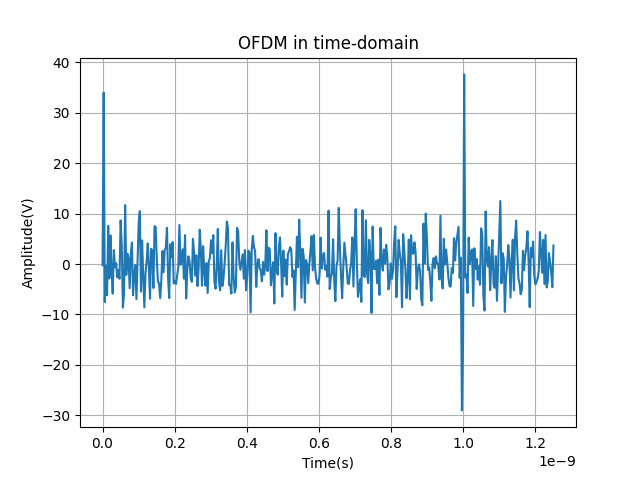
\includegraphics[width=\linewidth]{../Source/results/time_domain_1}
        \caption{Time Domain}
        \label{time-domain}
    \end{subfigure}
    \hfil
    \begin{subfigure}[t]{0.49\linewidth}
        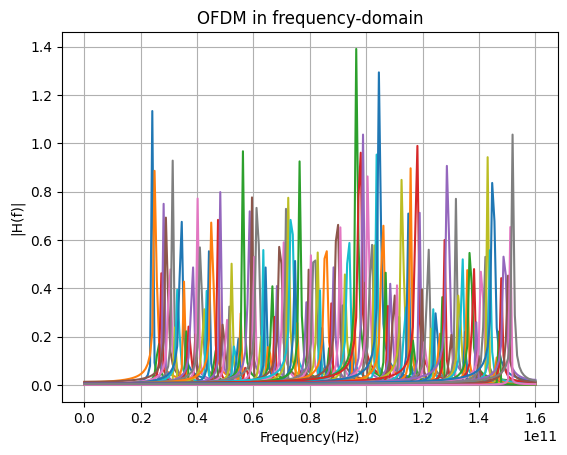
\includegraphics[width=\linewidth]{../Source/results/freq_domain_1}
        \caption{Frequency Domain}
        \label{freq-domain}
    \end{subfigure}
    \caption{OFDM\_data in time domain and frequency domain}
    \label{time-freq}
\end{figure}

Subsequently, we add a cyclic prefix to the symbol. This operation concatenates a copy of the last CP samples of the OFDM time domain signal to the beginning. This way, a cyclic extension is achieved. The CP fulfills two tasks:
\begin{enumerate}
    \item It isolates different OFDM blocks from each other when the wireless channel contains multiple paths, i.e. is frequency-selective.
    \item It turns the linear convolution with the channel into a circular one. Only with a circular convolution, we can use the single-tap equalization OFDM.
\end{enumerate}

% After this step :
% \begin{itemize}
%     \item Number of OFDM carriers in frequency domain: 128
%     \item Number of OFDM samples in time-domain before CP: 128
%     \item Number of OFDM samples in time domain with CP: 160
% \end{itemize}

Now, the signal is sent to the antenna and sent over the air to the receiver. In between both antennas, there is the wireless channel. We model this channel as a static multipath channel with impulse response channelResponse. Hence, the signal at the receive antenna is the convolution of the transmit signal with the channel response. Additionally, we add some noise to the signal according to the given SNR value. Figure \ref{tx_rx} shows the TX and RX signal with SNRDB = 20db.

\begin{figure}[htbp]
    \centering
    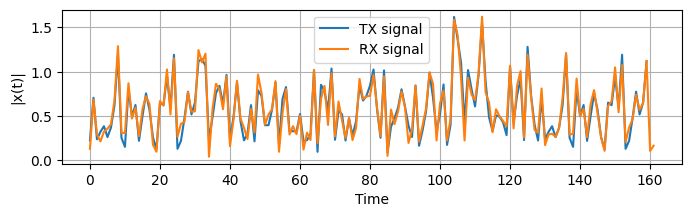
\includegraphics[width=\textwidth]{../Source/results/tx_rx}
    \caption{TX and RX signal with SNR value = 20db}
    \label{tx_rx}
\end{figure}

\subsection{OFDM Receiver}

Now, at the receiver the CP is removed from the signal and a window of $K$ samples is extracted from the received signal. Afterwards, the signal is transformed back to the frequency domain, in order to have the received value on each subcarrier available.

The principle of channel estimation is as follows:

The transmit signal contains pilot values at certain pilot carriers. These pilot values and their position in the frequency domain (i.e. the pilot carrier index) are known to the receiver. From the received information at the pilot subcarriers, the receiver can estimate the effect of the wireless channel onto this subcarrier (because it knows what was transmitted and what was received). Hence, the receiver gains information about the wireless channel at the pilot carriers. However, it wants to know what happened at the data carriers. To achieve this, it interpolates the channel values between the pilot carriers to get an estimate of the channel in the data carriers.

\begin{figure}[htbp]
    \centering
    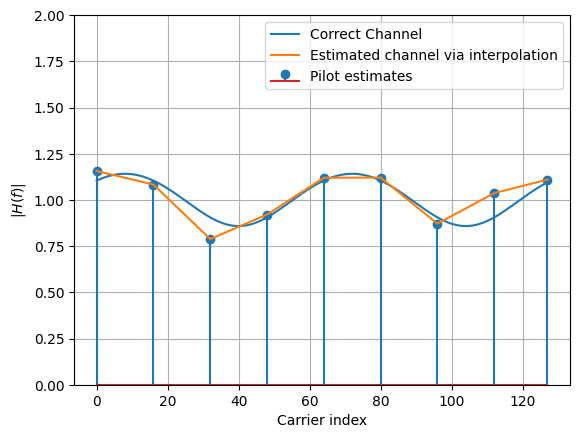
\includegraphics[width=\linewidth]{../Source/results/channel_estimation}
    \caption{The plot Correct Channel (blue) and estimated channel via interpolation (orange)}
    \label{channel_estimation}
\end{figure}

Now that the channel is estimated at all carriers, we can use this information in the channel equalizer step. Here, for each subcarrier, the influence of the channel is removed such that we get the clear (only noisy) constellation symbols back. The next step is to extract the data carriers from the equalized symbol. Here, we throw away the pilot carriers, as they do not provide any information, but were used for the channel estimation process.

\begin{figure}[htbp]
    \centering
    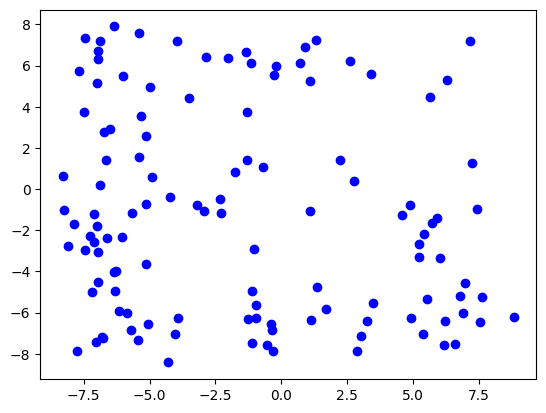
\includegraphics[width=\linewidth]{../Source/results/data_carriers}
    \caption{Received constellation}
    \label{received}
\end{figure}

Now, that the constellation is obtained back, we need to send the complex values to the demapper, to transform the constellation points to the bit groups. In order to do this, we compare each received constellation point against each possible constellation point and choose the constellation point which is closest to the received point. Then, we return the bit-group that belongs to this point. In the Figure \ref{hard-decision}, the blue points are the received QAM points, where as the the red points connected to them are the closest possible constellation points, and the bit groups corresponding to these red points are returned.

\begin{figure}[htbp]
    \centering
    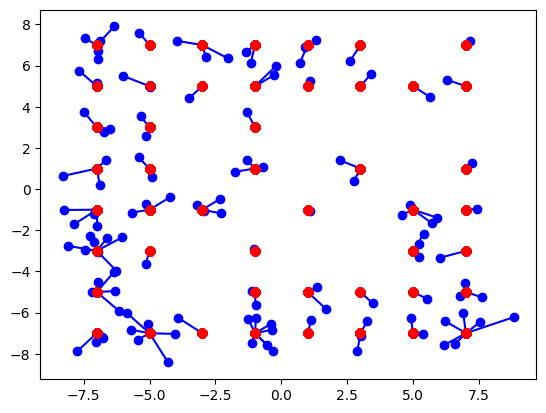
\includegraphics[width=\linewidth]{../Source/results/demapping}
    \caption{Hard Decision demapping}
    \label{hard-decision}
\end{figure}

Finally, the bit groups need to be converted to a serial stream of bits, by means of parallel to serial conversion. Figure \ref{output} show The received data for 4 cases of SRN equals 0, 10, 20 and 30 db respectively. Additionally, Table \ref{errors} show the calculated error bits using CRC check.

\begin{figure}[htbp]
    \centering
    \begin{subfigure}[t]{.49\linewidth}
        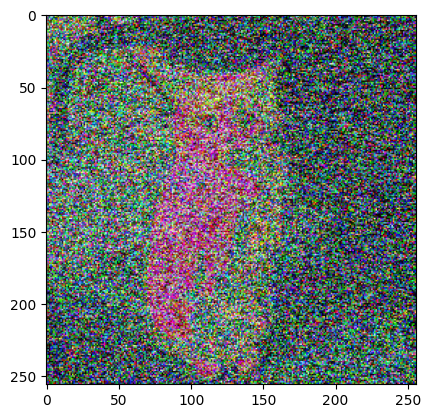
\includegraphics[width=\linewidth]{../Source/results/output_0db}
        \caption{SNR = 0db}
        \label{0db}
    \end{subfigure}
    \hfil
    \begin{subfigure}[t]{0.49\linewidth}
        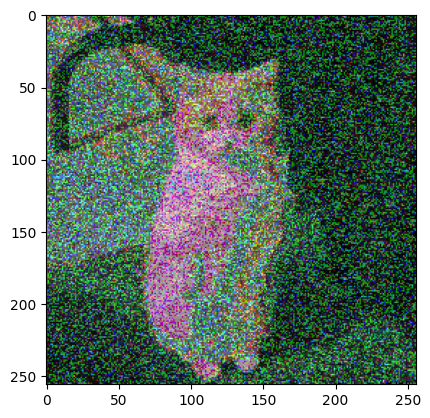
\includegraphics[width=\linewidth]{../Source/results/output_10db}
        \caption{SNR = 10db}
        \label{10db}
    \end{subfigure}
    \hfil
    \begin{subfigure}[t]{0.49\linewidth}
        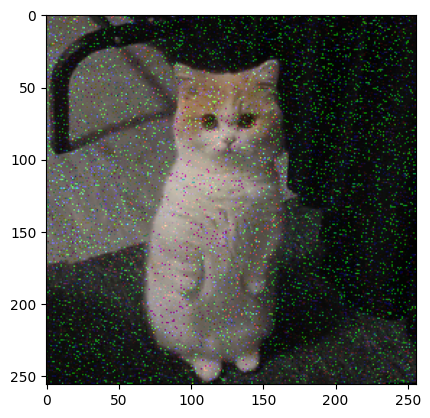
\includegraphics[width=\linewidth]{../Source/results/output_20db}
        \caption{SNR = 20db}
        \label{20db}
    \end{subfigure}
    \hfil
    \begin{subfigure}[t]{0.49\linewidth}
        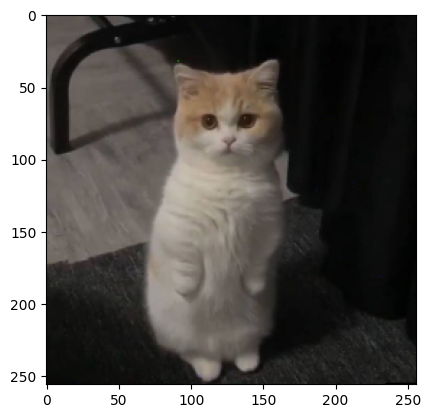
\includegraphics[width=\linewidth]{../Source/results/output_30db}
        \caption{SNR = 30db}
        \label{30db}
    \end{subfigure}
    \caption{The received using 64 QAM module}
    \label{output}
\end{figure}

\begin{table}[htbp]
    \centering
    \begin{tabular}{|c|c|c|}
        \hline
        SNR (db) & Total bits & Error bits \\ \hline
        0        & 2162706    &  171985 \\ \hline
        10       & 2162706    &  166022 \\ \hline
        20       & 2162706    &  51401  \\ \hline
        30       & 2162706    &  55     \\ \hline
    \end{tabular}
    \caption{Total bits and Error bits at 4 values of SNR}
    \label{errors}
\end{table}

For further analysis, we the varying SNRDB from 0 to 40 db and plot the equivalent BER value, as shown in Figure \ref{ber}.

\begin{figure}[htbp]
    \centering
    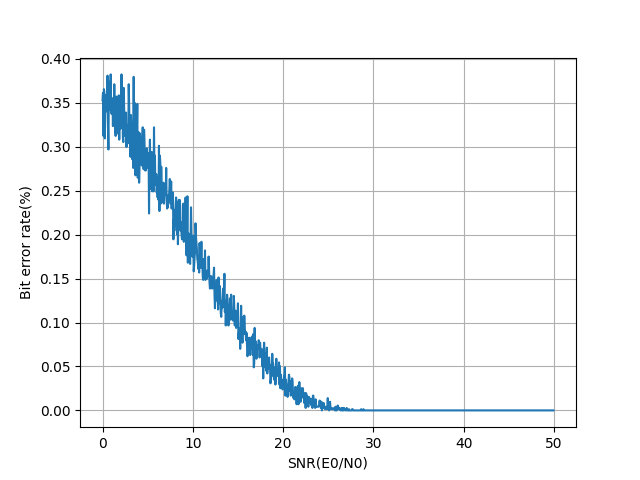
\includegraphics[width=\linewidth]{../Source/results/ber}
    \caption{Plot of BER for SNRdb values from 0 to 40}
    \label{ber}
\end{figure}

% \begin{table}[htbp]
%     \centering
%     \begin{tabular}{|c|c|}
%         \hline
%         Parameters & Values \\
%         \hline
%         Source Image Size & 256x256 \\
%         \hline
%     \end{tabular}
% \end{table}